\documentclass[border=10pt]{standalone}
\usepackage{tikz}
\usetikzlibrary{calc}

\begin{document}
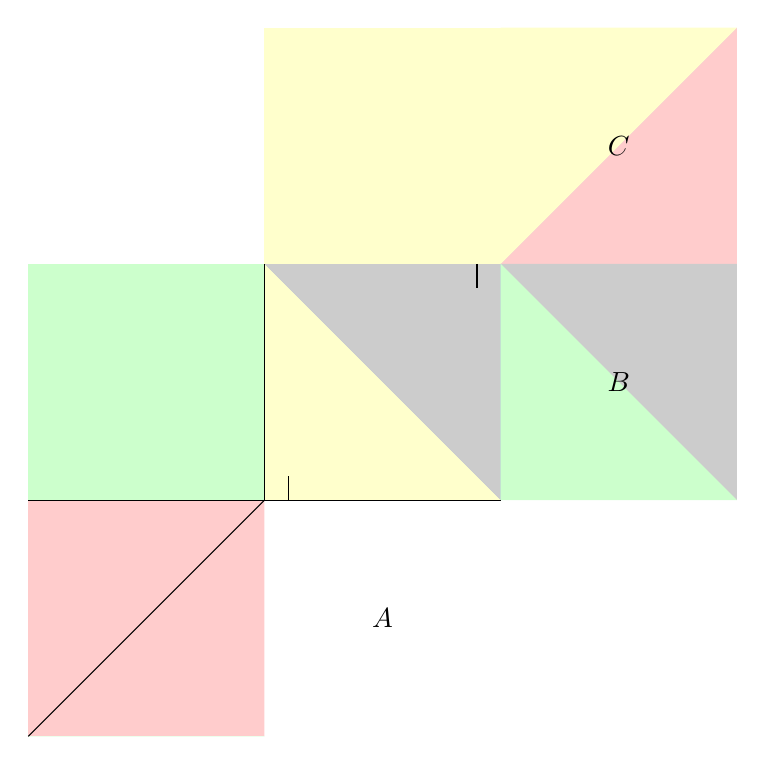
\begin{tikzpicture}[scale=1.5]
    % Define colors
    \definecolor{lightblue}{RGB}{173, 216, 230}
    \definecolor{pink}{RGB}{255, 204, 204}
    \definecolor{yellow}{RGB}{255, 255, 204}
    \definecolor{gray}{RGB}{204, 204, 204}
    \definecolor{green}{RGB}{204, 255, 204}

    % Central square
    \fill[lightblue] (0,0) rectangle (2,2);

    % Surrounding triangles
    \fill[pink] (-2,0) -- (0,0) -- (0,-2) -- cycle;
    \fill[yellow] (2,0) -- (0,0) -- (0,2) -- cycle;
    \fill[gray] (0,2) -- (2,2) -- (2,0) -- cycle;
    \fill[green] (0,-2) -- (-2,-2) -- (-2,0) -- cycle;

    % Outer squares
    \fill[pink] (-2,-2) rectangle (0,0);
    \fill[yellow] (0,2) rectangle (2,4);
    \fill[gray] (2,0) rectangle (4,2);
    \fill[green] (-2,0) rectangle (0,2);

    % Dividing lines in outer squares
    \draw (0,0) -- (-2,-2);
    \draw (0,0) -- (0,2);
    \draw (0,0) -- (2,0);
    \draw (0,0) -- (-2,0);

    % Additional square C
    \fill[lightblue] (2,2) rectangle (4,4);
    \fill[pink] (2,2) -- (4,2) -- (4,4) -- cycle;
    \fill[yellow] (2,2) -- (2,4) -- (4,4) -- cycle;
    \fill[gray] (2,2) -- (4,2) -- (4,0) -- cycle;
    \fill[green] (2,2) -- (2,0) -- (4,0) -- cycle;

    % Labels
    \node at (1,-1) {$A$};
    \node at (3,1) {$B$};
    \node at (3,3) {$C$};

    % Right angle marks
    \draw (0,0) ++(0.2,0) |- ++(0,0.2);
    \draw (2,2) ++(-0.2,0) |- ++(0,-0.2);
\end{tikzpicture}
\end{document}